\subsection{Gate-based Quantum Computing}

In the gate-based model of quantum computers, gates represent the manipulation of qubits.
The qubits and quantum gates form a quantum circuit.

Single qubit gates manipulate only one qubit at a time.
Double qubit gates manipulate two qubits and can entangle two qubits.
The formula (\ref{formula:gate.x}) shows an example of a single qubit gate.
It swaps the amplitudes of the two basis states $\ket{0}$ and $\ket{1}$.
The formula (\ref{formula:gate.cnot}) shows an example of a double qubit gate.
It applies the $X$-gate to the second qubit if the first qubit is in the base state $\ket{1}$.
This entangles both qubits with each other.
\begin{subequations}
\begin{align}
  \label{formula:gate.x}
  X & = \ket{0} \bra{1} + \ket{1} \bra{0}
  & = \begin{pmatrix}
    0 & 1 \\ 1 & 0
  \end{pmatrix}
  \\
  \label{formula:gate.hadamard}
  H & = \frac{1}{\sqrt{2}} \left(
    \left( \ket{0} + \ket{1} \right) \bra{0}
    + \left( \ket{0} - \ket{1} \right) \bra{0}
  \right)
  & = \frac{1}{\sqrt{2}} \begin{pmatrix}
    1 & 1 \\ 1 & -1
  \end{pmatrix}
  \\
  \label{formula:gate.cnot}
  CNOT & = \ket{00} \bra{00} + \ket{01} \bra{01} + \ket{10} \bra{11} + \ket{11} \bra{10}
  & = \begin{pmatrix}
    1 & 0 & 0 & 0 \\
    0 & 1 & 0 & 0 \\
    0 & 0 & 0 & 1 \\
    0 & 0 & 1 & 0
  \end{pmatrix}
\end{align}
\end{subequations}

A quantum circuit consists of one or more quantum gates that are operating on one or more qubits.
The quantum circuit \ref{figure:gate.deutsch.circuit} depicts the Deutsch algorithm for the function $f: x \mapsto x$.
The dot with the line to the circled plus stands for the $CNOT$ gate, and the $H$ gates stand for Hadamard gates.
A Hadamard gate puts qubits that are in a basis state into a superposition where both outcomes of the measurement are equally likely.
It is described by the formula (\ref{formula:gate.hadamard}).
The last gate stands for a measurement.
In this case only the first qubit gets measured.
\cite{Deutsch1985}
\begin{figure}[!h]
  \centering
  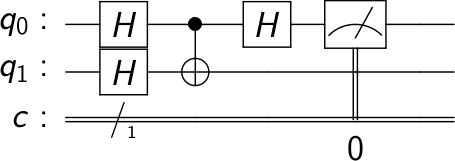
\includegraphics[width=0.5 \textwidth]{02_Background/deutsch_algorithm_circuit.png}
  \caption{Deutsch Algorithm for $f: x \mapsto x$}
  \label{figure:gate.deutsch.circuit}
\end{figure}

A quantum computer that implements this model of computing would be more powerful than any Turing machine.
It can simulate any finite physical system with polynomial time complexity, including systems with quantum effects.
The complexity class is called Bounded-error Quantum Polynomial-time (BQP).
There exists no known algorithm for Turing machines to accomplish this.
\cite{Deutsch1985, Shor1998}

\subsubsection{Grover Algorithm}

The Grover Algorithm is a quantum algorithm for unstructured search.
It can find an element that satisfies some condition $C$ in an unstructured list with the time complexity of $O(\sqrt{n})$.
\cite{Grover1996}
If multiple elements satisfy the condition, only one of those elements can be found in one execution of the algorithm.
\cite{Boyer1998}

The algorithm consists on 3 parts:
\begin{enumerate}
  \item Initialize the input register with the equal superposition $\ket{\Phi} = \frac{1}{\sqrt{N}} \sum_{x=0}^N \ket{x}$
  \item \label{backg:quantum.grover.iteration}
  Repeat the following steps $O(\sqrt{N})$ times:
  \begin{enumerate}[label=\alph*)]
    \item Rotate all states that satisfy $C$ by $\pi$.
    \item Apply the diffusion operator $D$.
    It is defined as \begin{align}
      D_{i, j} = \begin{cases}
        \frac{2}{N} & i \neq j\\
        \frac{2}{N} - 1 & else
      \end{cases}
    \end{align}
  \end{enumerate}
  \item \label{backg:quantum.grover.sampling}
  Sample the input register.
\end{enumerate}

Step \ref{backg:quantum.grover.iteration} is called the Grover-iteration $G$.
Its first part that rotates desired states is called an oracle.
The Grover-iteration amplifies the amplitudes of desired states.
This increases the probability of measuring those states in step \ref{backg:quantum.grover.sampling}.
\cite{Grover1996}

\subsubsection{Optimization}

Optimizing QUBOs on gate-based quantum computers is possible by iteratively searching for better values of the QUBO variables.
The algorithm uses the Grover search to search for better values for the QUBO variables.
It uses two quantum registers to represent the variables of the QUBO ($\ket{x}$) and the energy value of the QUBO ($\ket{z}$).
\cite{Gilliam2019}

The oracle consists of multiple rotations of qubits of $\ket{z}$.
The qubits of $\ket{x}$ control the rotations.
The rotations add the biases of the QUBO to the value of the quantum register in the Fourier-domain.
After that, the oracle subtracts the current minimum energy value $y$ from the value of $\ket{z}$.
The inverse Fourier-transformation converts the $\ket{z}$ register to a Two's Complement basis.
The most significant qubit of $\ket{z}$ signals the sign of the value and controls the typical oracle used to rotate the desired states.
\cite{Gilliam2019}

This way, the measurement of $\ket{x}$ yields values for the QUBO variables that correspond to a lower energy value $y'$ than the minimum found before $y$.
In the next iteration, the oracle subtracts $y'$ from $\ket{z}$ after adding the biases.
By repeating this process, the algorithm identifies the values for the QUBO variables that minimize the energy.
\cite{Gilliam2019}
